% !TEX root = main.tex

%%%%%%%%%%%%%%%%%%%%%%%%%%%%%%%%%%%%%%%%%%%%%%%%%%%%%%%%%%%%%%%%%%%%%%%%%%%%%%%%%%%%%%%%%%%%%%%%
\section{原理}
%%%%%%%%%%%%%%%%%%%%%%%%%%%%%%%%%%%%%%%%%%%%%%%%%%%%%%%%%%%%%%%%%%%%%%%%%%%%%%%%%%%%%%%%%%%%%%%%

\subsection{ソレノイドによる磁場}
図1のような半径$a$,長さ$b$の円筒ソレノイドによって中心軸上$(r = 0)$のP点に
作られる$B_z$は,単位長さあたりの巻数を$n$,ソレノイドに流れる電流を$I$とすると,
$$
B_z=\frac{\mu_0 n I}{2}(\cos \theta_2 - \cos \theta_1)
$$
であるから,ソレノイドのそう巻き数をN$(=nb)$,左側からP点までの距離を$z$とすると,
$$
\cos \theta_1 = \frac{z-b}{\sqrt[]{a^2+(z-b)^2}}\quad,\quad \cos \theta_2 = \frac{z}{\sqrt[]{a^2+z^2}}
$$
であるから,
$$
B_z=\frac{\mu_0 NI}{2} \{ \frac{z}{\sqrt[]{a^2+z^2}} + \frac{b-z}{\sqrt[]{a^2+(z-b)^2}} \}
$$
となる.
\begin{figure}[!ht]
    \centering
    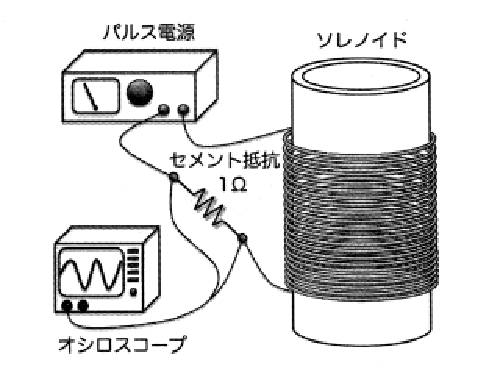
\includegraphics[scale=0.75]{figure1.pdf}
    \caption{有限長ソレノイド}
\end{figure}

